\documentclass{article}
\usepackage{graphicx}
\usepackage[margin=1in]{geometry}
\usepackage[outdir=./]{epstopdf}  					% Avoids errors when input figures
\usepackage[labelsep=period,labelfont=bf]{caption}
%\usepackage{afterpage}
%\usepackage{subcaption}

\begin{document}
%	\afterpage{
	\begin{figure}[t]
		\caption{Monetary Policy Dimensions} \label{fig:factorspoints}
		\begin{center}								% center the minipage on the line
			\begin{minipage}{0.9\linewidth}
				\begin{center}							% center the figure inside the minipage
%					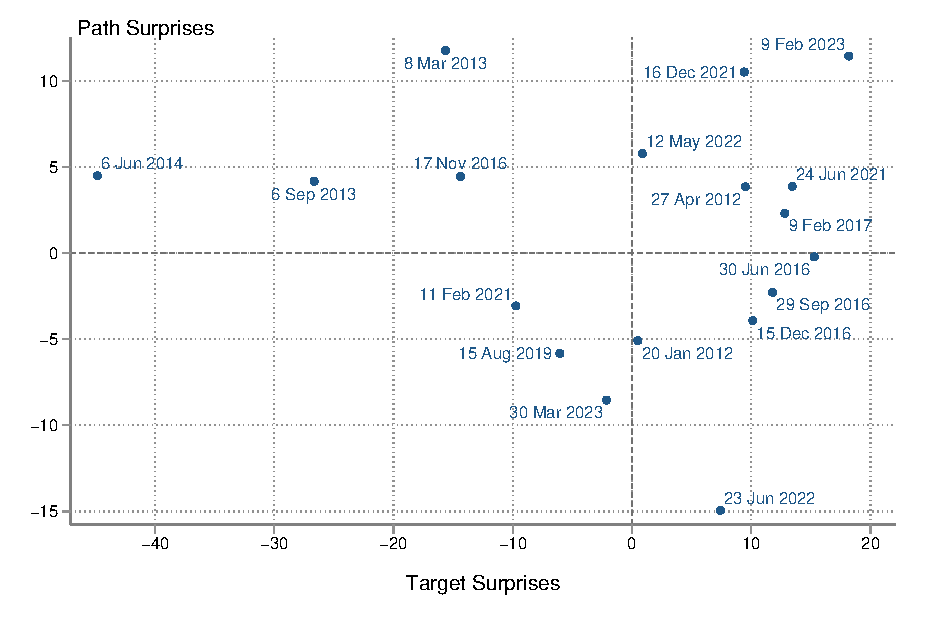
\includegraphics[width=1\textwidth,height=.4\textheight]{../Figures/factorspointstg.eps} \\
%					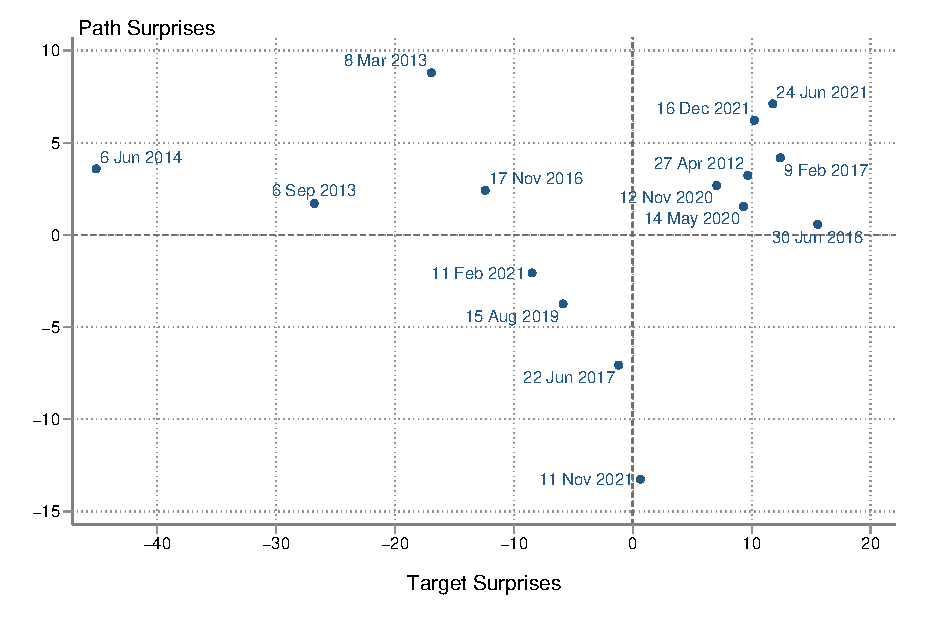
\includegraphics[width=1\textwidth,height=.4\textheight]{../Figures/factorspointswd.eps} \\
%					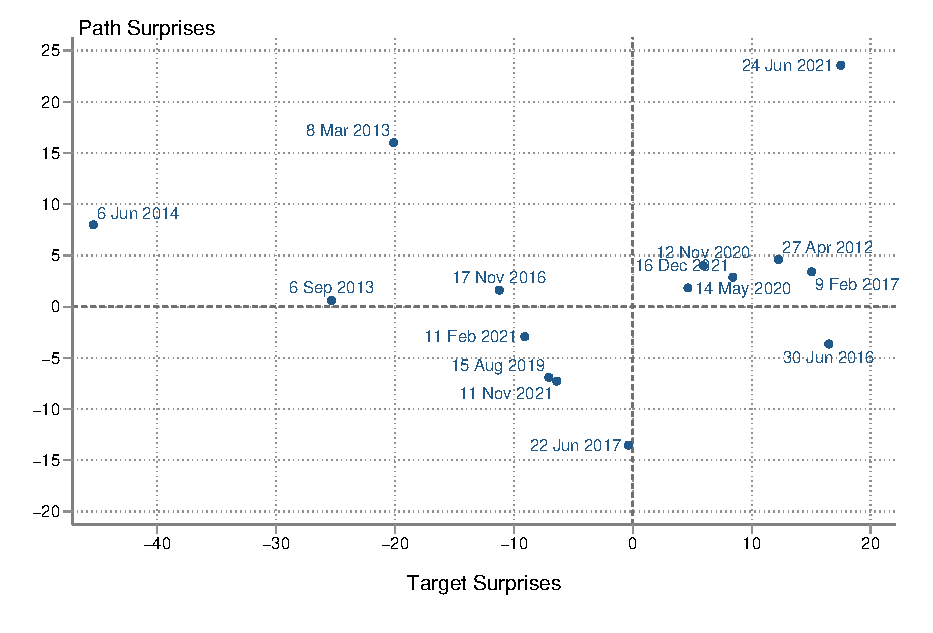
\includegraphics[width=1\textwidth,height=.4\textheight]{../Figures/factorspointsdy.eps} \\
					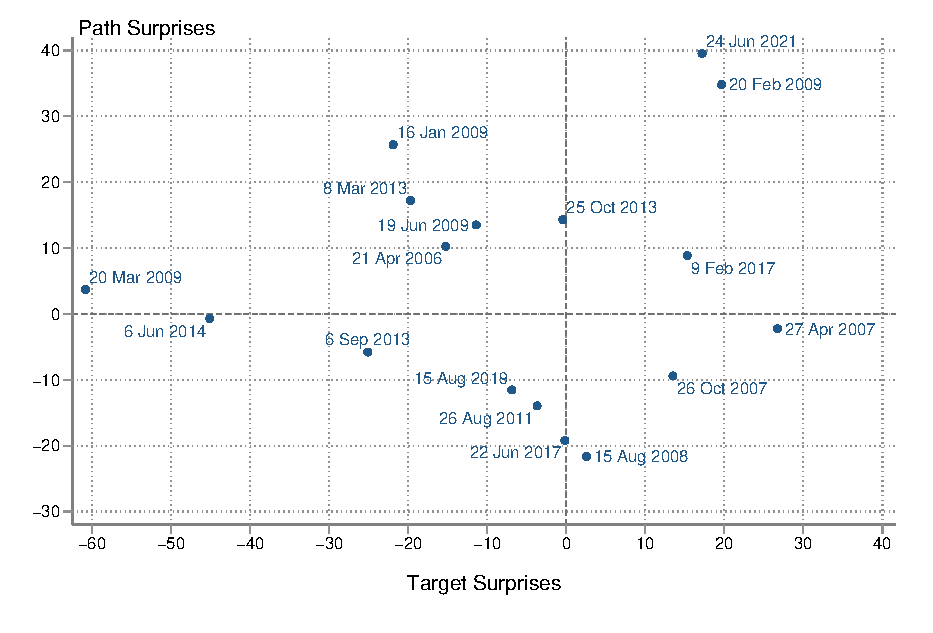
\includegraphics[width=1\textwidth,height=.4\textheight]{../Figures/factorspoints04.eps} \\
				\end{center}
				\vspace{-0.4cm}
				\fignotes{This figure plots the largest estimated target and path surprises (expressed in basis points) obtained from daily data, as explained in the main text. The sample includes all regular monetary policy announcements from January 2004 to \lastobs.} 
			\end{minipage}
		\end{center}
	\end{figure}
%	}
\end{document}
% trim = {<left> <lower> <right> <upper>}
